\documentclass[12pt, fullpage,letterpaper]{article}

\usepackage[margin=1in]{geometry}
\usepackage{url}
\usepackage{amsmath, amsthm, amssymb}
\usepackage{booktabs}
\usepackage{pgfplotstable}
\usepackage{tikz-cd}
\usepackage{tikz}
\usetikzlibrary{arrows, positioning}


\newcommand{\semester}{Spring 2024}
\newcommand{\assignmentId}{4}
\newcommand{\releaseDate}{March 15, 2020}
\newcommand{\dueDate}{March 29, 2020}

\newcommand{\bx}{{\bf x}}
\newcommand{\bw}{{\bf w}}
\DeclareMathOperator{\sgn}{sgn}

\pgfplotsset{my style/.append style={axis x line=middle, axis y line=
middle, xlabel={$x$}, ylabel={$y$}, axis equal }}

\title{CS 5350/6350, DS 4350: Machine Learning \semester}
\author{Homework \assignmentId}
  
\begin{document}

\maketitle
\begin{center}
	\text{Author: Jordy A. Larrea Rodriguez}
\end{center}

% \section*{General Instructions}

{\footnotesize
  \begin{itemize}
  \item You are welcome to talk to other members of the class about
    the homework. I am more concerned that you understand the
    underlying concepts. However, you should write down your own
    solution. Please keep the class collaboration policy in mind.

  \item Feel free discuss the homework with the instructor or the TAs.

  \item Your written solutions should be brief and clear. You need to
    show your work, not just the final answer, but you do \emph{not}
    need to write it in gory detail. Your assignment should be {\bf no
      more than 10 pages}. Every extra page will cost a point.

  \item Handwritten solutions will not be accepted.

  \item The homework is due by midnight of the due date. Please submit
    the homework on Canvas. You should upload one file: a PDF report with answers to the questions below.

  \item Some questions are marked {\bf For 6350 students}. Students who are
    registered for CS 6350 should do these questions. Of course, if you are
    registered for CS 5350 or DS 4350, you are welcome to do the question too,
    but you will not get any credit for it.

  \end{itemize}

 \paragraph{Important.} Do not just put down an answer. We want an
  explanation. No points will be given for just the final answer
  without an
  explanation. You will be graded on your reasoning, not just
   on your final result.

   Please follow good proof technique; what this means is if you make
   assumptions, state them. If what you do between one step and the
   next is not trivial or obvious, then state how and why you are
   doing what you are doing. A good rule of thumb is if you have to
   ask yourself whether what you are doing is obvious, then it is
   probably not obvious. Try to make the proof clean and easy to
   follow. 
}


\section{PAC Learnability of Depth Limited Decision Trees [30 points]}
\label{sec:pac-learn-depth}


In this question, you will be showing that depth limited decision trees are PAC
learnable.

Suppose we have a binary classification problem with $n$ Boolean features that
we seek to solve using decision trees of depth $k$. For this question assume trees are complete, meaning each node (other than the leaf nodes) has exactly two children. The figure below shows some
examples of such trees and their depths. 

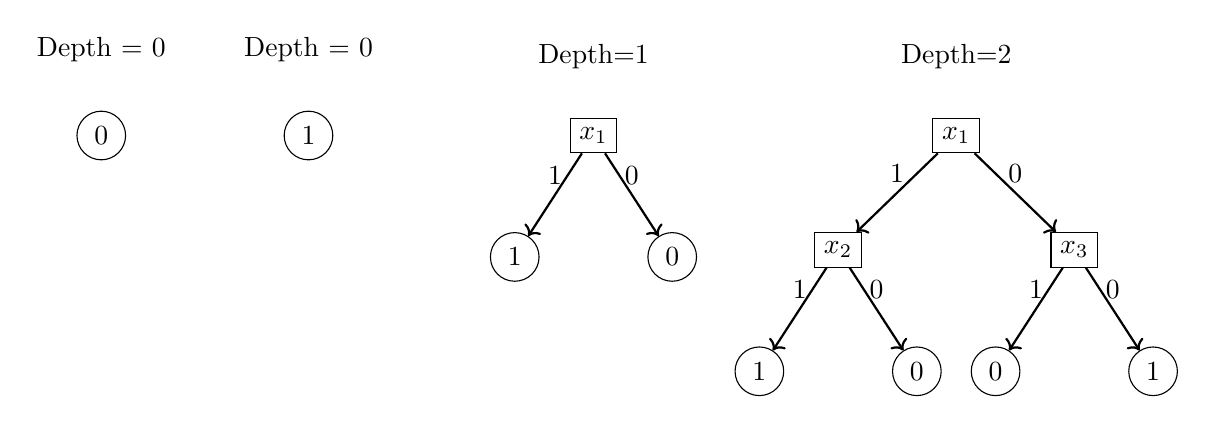
\begin{tikzpicture}
  \node[draw, circle] (false) at (0,0) {$0$};
  \node[above=0.5cm of false] {Depth = 0};

  \node[draw, circle, right=2cm of false] (true)  {$1$};
  \node[above=0.5cm of true] {Depth = 0};

  \node[draw, rectangle, right=3cm of true] (t21) {$x_1$};
  \node[draw, circle, below=1cm of t21, xshift=-1cm] (t22) {$1$};
  \node[draw, circle, below=1cm of t21, xshift=1cm] (t23) {$0$};
  \draw[->,thick] (t21) -- node[midway, above] {$1$} (t22);
  \draw[->,thick] (t21) -- node[midway, above] {$0$} (t23);  

  \node[above=0.5cm of t21] {Depth=1};

  \node[draw, rectangle, right=4cm of t21] (t31) {$x_1$};
  \node[draw, rectangle, below=1cm of t31, xshift=-1.5cm] (t32) {$x_2$};
  \node[draw, rectangle, below=1cm of t31, xshift=1.5cm] (t33) {$x_3$};
  \node[draw, circle, below=1cm of t32, xshift=-1cm] (t34) {$1$};
  \node[draw, circle, below=1cm of t32, xshift=1cm] (t35) {$0$};
  \node[draw, circle, below=1cm of t33, xshift=-1cm] (t36) {$0$};
  \node[draw, circle, below=1cm of t33, xshift=1cm] (t37) {$1$};

  \draw[->,thick] (t31) -- node[midway, above] {$1$} (t32);
  \draw[->,thick] (t31) -- node[midway, above] {$0$} (t33);

  \draw[->,thick] (t32) -- node[midway, above] {$1$} (t34);
  \draw[->,thick] (t32) -- node[midway, above] {$0$} (t35);
  \draw[->,thick] (t33) -- node[midway, above] {$1$} (t36);
  \draw[->,thick] (t33) -- node[midway, above] {$0$} (t37);    
  \node[above=0.5cm of t31] {Depth=2};  
\end{tikzpicture}

\begin{enumerate}
\item Since decision trees represent a finite hypothesis class, the quantity of
  interest is the number of such trees---i.e., trees with depth $k$ over $n$
  features. Suppose we use $S_n(k)$ to denote the number of the number of trees
  with depth exactly $k$ if we have $n$ features.

  The following questions guide you through this counting process. Recall that
  each answer should be accompanied with an explanation.\emph{If you simply
    write the final answer, you will not get any points.} (\textbf{Please see the note at the end of this questions for further clarification}3).

  \begin{enumerate}
  \item \relax[2 points] What is $S_n(0)$? That is how many trees of depth $0$
    exist? \newline
    
    \textbf{Response:} $S_n(0) = 2$, there are two trees which can be visualized in the figure above for Depth = 0.
    
  \item \relax[3 points] What is $S_n(1)$? That is, with $n$ features, how many
    trees of depth $1$ exist? \newline
    
    \textbf{Response:} $S_n(1) = n(2^2-1) = 3n$, there are exactly $n$ different features that $x_i$ can take; furthermore, there are $2^2-1$ different leaf nodes since the binary string $\{01\}$ is structurally the same as $\{10\}$. 
    
  \item \relax[4 points] Suppose you know the number of trees with depth $i$,
    for some $i$. This quantity would be $S_n(i)$ using our notation. Write down
    a recursive definition for $S_n(i+1)$ in terms of $n$ and $S_n(i)$.

    For this expression, you can assume that we are allowed to the use same
    feature any number of times when the tree is constructed. \newline
    
    \textbf{Response:} We know that $Sn(1) = 3n$.
    For $i = 2$, we have $2^4=16$ different leaf nodes: so 16-1 unique enumerations at the leafs. We can take the permutation at depth 1 to count the different enumerations possible that is count = $_n P_2 = \frac{n!}{(n-2)!} = n(n-1)$. At the root we have the same $n$ different enumerations. Recursively this can be written as, $$S_n(2)=S_n(1) \times 5n(n-1)$$
    Following the same pattern for $i=3$, we obtain, $$S_n(3)=S_n(2) \times 17 \frac{n!}{(n-4)!}$$
    And again for $i=4$: $$S_n(4) = S_n(3) \times 257 \frac{n!}{(n-8)!}$$
    Thus, the recursive formula follows,
    $$S_n(i+1) = S_n(i) \times \frac{2^{2^{i+1}}-1}{2^{2^i}-1} \frac{n!}{(n-2^i)!}$$

  \item \relax[6 points] Recall that the quantity of interest for PAC bounds is
    the $\log$ of the size of the hypothesis class. Using your answer for the
    previous questions, find a closed form expression representing $\log S_n(k)$
    in terms of $n$ and $k$. Since we are not looking for an exact expression,
    but just an order of magnitude, so you can write your answer in the big $O$
    notation. \newline 
    
    \textbf{Response:} From part (c) above: $$S_n(k) = S_n(k-1) \times \frac{2^{2^{k}}-1}{2^{2^{k-1}}-1} \frac{n!}{(n-2^{k-1})!}$$
    
    Taking the base 2 log of $S_n(k)$ and simplifying, 
    $$lg(S_n(k)) = lg(S_n(k-1)) + (lg({2^{2^k}-1})-lg(2^{2^{k-1}}-1)) + lg(\frac{n!}{(n-2^{k-1})!})$$
    
    Clearly, the first and second terms are not major contributors when taking the limit for a big enough k and n. Thus, $$lg(S_n(k)) \approxeq lg(\frac{n!}{(n-2^{k-1})!})$$
    
    It is clear by considering properties of the factorial operator that $\frac{n!}{(n-2^{k-1})!} < n^{2^k}$. Therefore, we can declare that, $$lg(S_n(k)) < lg(n^{2^k})$$
    Finally, we can attest that $S_n(k)$ is in the order of $O(2^k \: lg(n))$.
  \end{enumerate}

\item Next, you will use your final answer from the previous question to state a
  sample complexity bound for decision trees of depth $k$.

  \begin{enumerate}
  \item \relax[3 points] With finite hypothesis classes, we saw two Occam's
    razor results. The first one was for the case of a consistent learner and
    the second one was for the agnostic setting. For the situation where we are
    given a dataset and asked to use depth-$k$ decision trees as our hypothesis
    class, which of these two settings is more appropriate? Why?
    
    \textbf{Response:} 
    The Agnostic approach to Occam’s Razor fits better here. Decision trees with fixed depths might not always capture real-world data complexity. Staying open to the possibility that the true target function lies beyond depth-k trees allows exploring more hypotheses, potentially improving generalization.

  \item \relax[4 points] Using your answers from questions so far, write the
    sample complexity bound for the number of examples $m$ needed to guarantee
    that with probability more than $1- \delta$, we will find a depth-$k$
    decision tree whose generalization error is no more than $\epsilon$ away
    from its training error.\newline
	\textbf{Response:} From lecture we know that the number of samples $m$ is lower bounded such that, $m \geq \frac{1}{\epsilon ^2}(ln(|H|)+ln(\frac{1}{\sigma}))$, where $|H| = n^{2^k}$. Thus, $$m \geq \frac{1}{\epsilon ^2}(2^k ln(n)+ln(\frac{1}{\sigma}))$$
  \end{enumerate}

\item \relax[4 points] Is the set of depth-$k$ decision trees PAC learnable? Is
  it efficiently PAC learnable? \newline
  
  \textbf{Response:} For depth $k$ decision trees, the hypothesis class is clearly PAC learnable given the big O. Furthermore, the hypothesis class is clearly efficiently PAC learnable since a variety of algorithms exist that solve the problem. For example, the ID3 algorithm is proven to be NP-complete and is in the order of $O(m \times n)$ for $n$ binary features and $m$ examples.

\item \relax[4 points] Suppose the number of features we have is large and the
  depth limit we are considering is also large (say, in the thousands or
  more). Will the number of examples we need be small or large? Discuss the
  implications of the sample complexity bound from above.
  
  \textbf{Response:} As the feature space and depth limit grow, the hypothesis class size $|H|$ tends to expand, potentially exponentially with tree depth. Consequently, the sample complexity $m$ required by the agnostic bound equation also increases. This suggests that a larger dataset is necessary to effectively learn decision trees with intricate structures and to ensure dependable generalization performance.
  
\end{enumerate}

\textbf{NOTE}: In this question we are counting trees that are structurally different instead of functionally different. As an exercise, you can confirm that the following two trees are structurally different but equal in terms of the label they assign to any example, namely the trees are functionally equivalent.


\begin{center}
    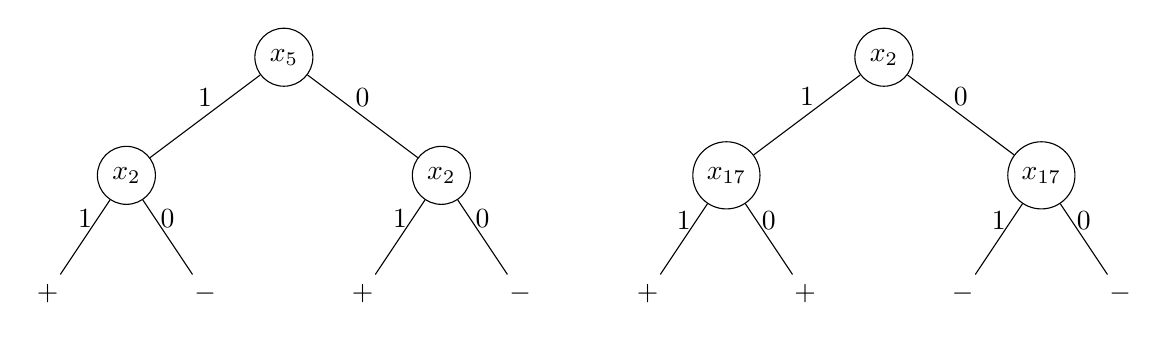
\begin{tikzpicture}[grow = down, level/.style={sibling distance=40mm/#1}, node/.style = {draw, circle}]
    \begin{scope}
      \node[node] {$x_5$} % root
      child { node[node] {$x_2$}
      child { node {$+$}
          edge from parent node [above] {1}}
      child { node {$-$}
          edge from parent node [above] {0}}
        edge from parent node [above] {1}}
      child { node[node] {$x_2$} % x_2
        child { node {$+$}
          edge from parent node [above] {1}}
        child { node {$-$}
          edge from parent node [above] {0}}
        edge from parent node [above] {0}};
    \end{scope}
    \begin{scope}[xshift=3in]
     \node[node] {$x_2$} % root
      child { node[node] {$x_{17}$}
      child { node {$+$}
          edge from parent node [above] {1}}
      child { node {$+$}
          edge from parent node [above] {0}}
        edge from parent node [above] {1}}
      child { node[node] {$x_{17}$} % x_2
        child { node {$-$}
          edge from parent node [above] {1}}
        child { node {$-$}
          edge from parent node [above] {0}}
        edge from parent node [above] {0}};
    \end{scope}
    \end{tikzpicture}
  \end{center}




\section{Shattering [15 points, for 6350 students]}
\label{sec:shattering}

Suppose we have a set $X_n$ consists of all binary sequences of a length $n$.
For example, if $n=3$, the set would consist of the eight elements
\texttt{\{000, 001, 010, 011, 100, 101, 110, 111\}}.

Consider a set of functions $H_n$ that we will call the set of {\em
  templates}. Each template is a sequence of length $n$ that is constructed
using {\tt 0}, {\tt 1} or {\tt -} and returns $+1$ for input binary sequences
that match it and $-1$ otherwise. While checking whether a template matches an
input, a {\tt -} can match both a {\tt 0} and a {\tt 1}.

For example, the template {\tt -10} matches the binary strings {\tt 010} and
{\tt 110}, while {\tt -1-} matches all strings that have a {\tt 1} in the middle
position, namely {\tt 010}, {\tt 011}, {\tt 110} and {\tt 111}.

Does the set of templates $H_n$ shatter the set $X_n$? Prove your answer. \newline

\textbf{Response:}
Suppose set $X_3$ consists of all binary strings of length n=3. Then, $X_3=\{\{000\}, \{001\}, ...,\{111\}\}$ and $|X_3|=8$. As stated in the example above $\{-1-\}$ matches 010, 011, 110, and 111. This can be generalized to state that a template w/ $k$ unique dashes can match $2^k$ different binary strings in $X_n$. Lets assume that $H_n$ has at least as many elements as $X_n$. The maximum size $|H_n|$ is $3^n$ which is larger than the length of $X_n$ or $2^n$. Because one template can match $2^k$ different binary strings of length $n$, we can realistically ensure that the set of templates $H_n$ can shatter the set $X_n$.

\section{VC Dimension [45 points]}
\label{sec:vc-dimension}
\begin{enumerate}
\item ~[5 points] Assume that the three points below can be labeled in any way.  Show with pictures how they can be shattered by a linear classifier.  Use filled dots to represent positive classes and unfilled dots to represent negative classes.

  \begin{tikzpicture}
    \begin{axis}[my style, xtick={-1,0,...,3}, ytick={-1,0,...,3},
      xmin=-1, xmax=3, ymin=-1, ymax=3]
      \addplot[mark=*,only marks] coordinates {(2,2)(1,1)(1,2)};
    \end{axis}
  \end{tikzpicture}
  
  \textbf{Response:} Refer to figure below for a visualization of a linear classifier shattering this dataset. \newline
  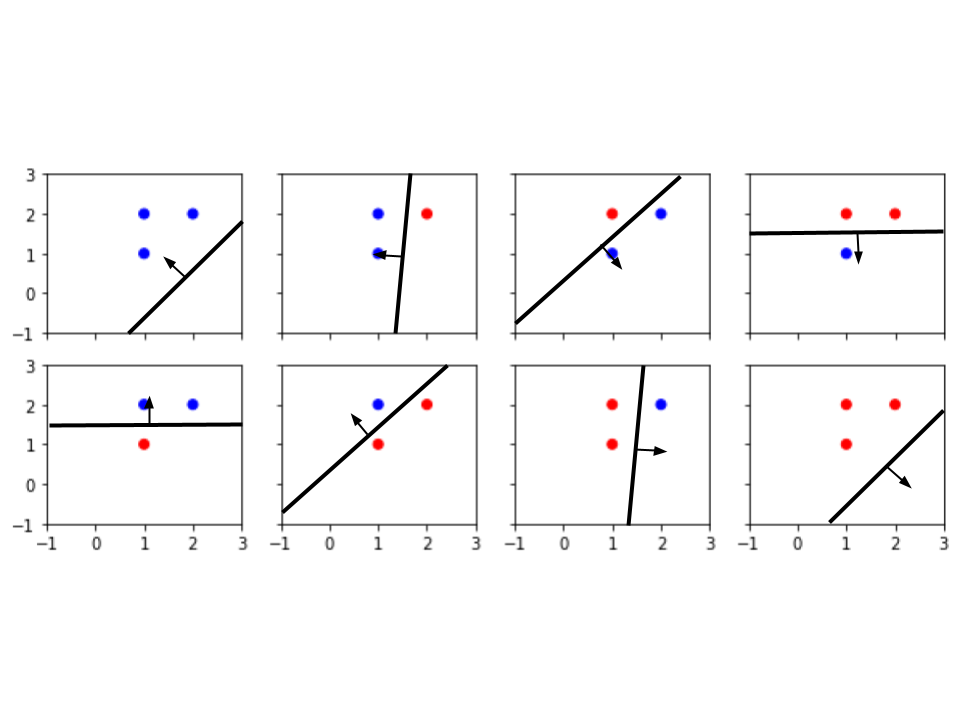
\includegraphics[scale=0.4]{./img/part3_1.png}
  
\item {\bf VC-dimension of axis aligned rectangles in $\mathbb{R}^d$}:
  Let $H^d_{rec}$ be the class of axis-aligned rectangles in
  $\mathbb{R}^d$. When $d=2$, this class simply consists of rectangles
  on the plane, and labels all points strictly outside the rectangle
  as negative and all points on or inside the rectangle as positive.
  In higher dimensions, this generalizes to $d$-dimensional boxes,
  with points outside the box labeled negative.

  \begin{enumerate}
  \item ~[10 points] Show that the VC dimension of $H^2_{rec}$ is 4.
  
  \textbf{Response:} To prove that the VC dimension of $H^2_{rec}$ is 4, $H^2_{rec}$ must shatter at least one subset of size 4 (ie, $VC(H^2_{rec}) \geq 4$) but there must not exist a single subset of size 5 that $VC(H^2_{rec})$ can shatter so $VC(H^2_{rec}) < 5$.
  \begin{enumerate}
  	\item ~Direct proof for $VC(H^2_{rec}) \geq 4$:
  	Below is a visualization showcasing how there exists at least one subset of size 4 that is shattered by $H^2_{rec}$.
  	
  	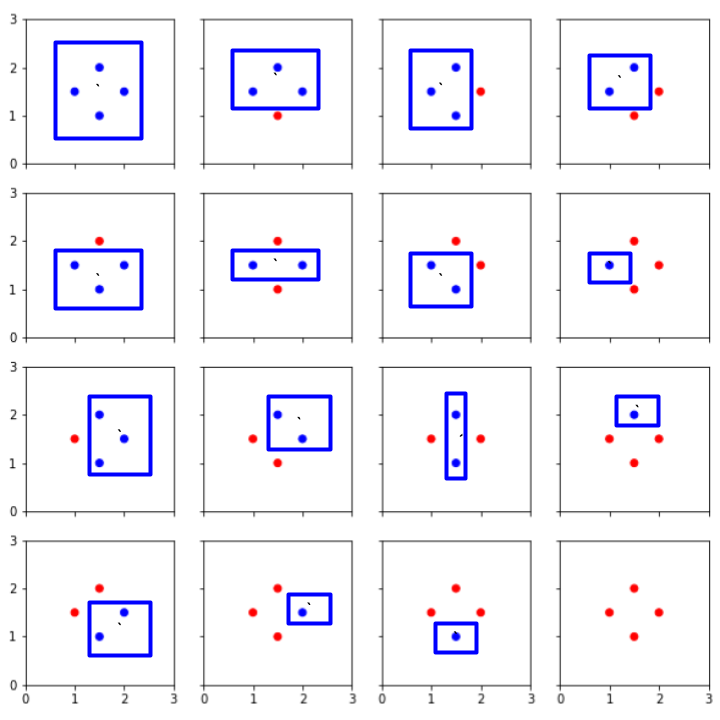
\includegraphics[scale=0.5]{./img/part3_2a1.png}
  	
  	\item ~Proof by contradiction for $VC(H^2_{rec}) < 5$:
  	For $VC(H^2_{rec}) >= 5$, there must exist at least one subset of size 5 that is shattered by $H^2_{rec}$. Let there be a set of four points $p_1, p_2, p_3, p_4,$ and $p_5$. Now consider two cases, case 1 where four points are enclosed and case 2 where only three points are within the rectangle.
  	\begin{enumerate}
  		\item[1.]{\textbf{Case 1:}} ~Let's assume that an axis-aligned rectangle correctly classifies $p_1, p_2, p_3$ and $p_4$ as positive and leaves $p_5$ outside the rectangle (labeled as negative). However, we can relabel the points such that 
  		$p_5$ is inside the rectangle, while the other four points are outside. This contradicts the assumption that the rectangle correctly classifies the points.
  		
  		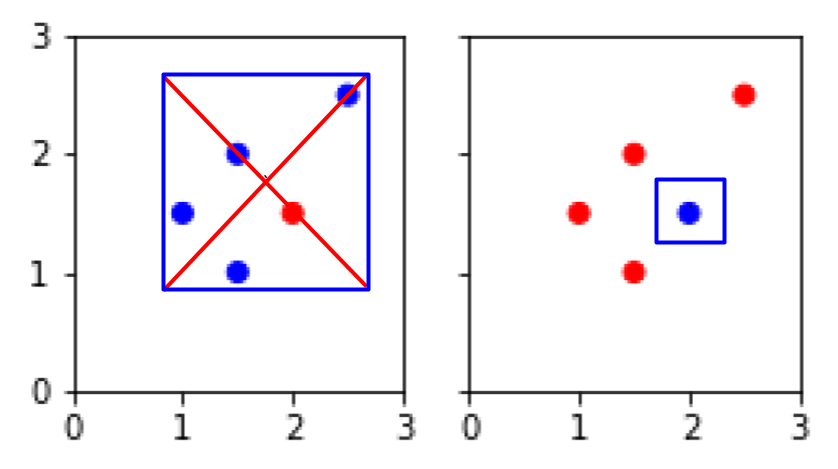
\includegraphics[scale=0.4]{./img/part3_2a2.png}
  		
  		\item[2.]{\textbf{Case 2:}} ~If an axis-aligned rectangle correctly classifies three points ($p_1, p_3,$ and $p_5$) as positive and two points as negative (remaining points), we can rearrange the points such that $p_2$ and $p_4$ are inside the rectangle while the rest are outside. Again, this contradicts the assumption.
  		
  		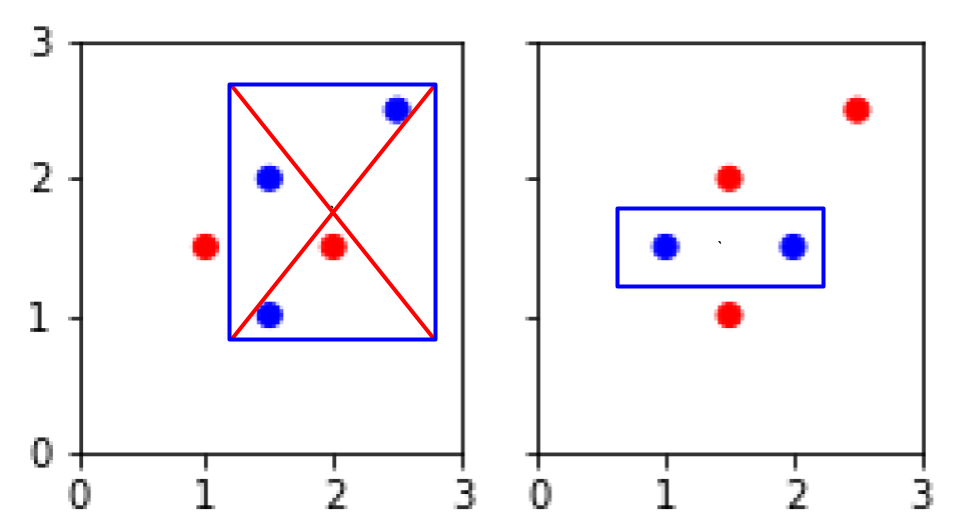
\includegraphics[scale=0.35]{./img/part3_2a3.png}
  	\end{enumerate}
  	Since no single rectangle can correctly classify all possible labelings of these five points, it's impossible to shatter a set of five points in $\mathbb{R}^2$.
  \end{enumerate}
  
  \item ~[10 points] Generalize your argument from the previous proof
    to show that for $d$ dimensions, the VC dimension of $H^d_{rec}$
    is $2d$.
    
	\textbf{Response:} To generalize on d-dimensions $H^d_{rec}$ must shatter at least one subset of size $2d$ (ie, $VC(H^d_{rec}) \geq 2d$) but there must not exist a single subset of size $2d+1$ that $VC(H^d_{rec})$ can shatter so $VC(H^d_{rec}) < 2d+1$.
	\newline
	Consider a set of points, each characterized by $d$ attributes. Each attribute can be positively or negatively labeled for each point. When we examine any subset of these points, we can always identify a rectangle that exclusively encompasses those points and not others. This observation establishes that the VC-dimension is at least $2d$. Now, let’s establish that the VC-dimension is less than $2d+1$. Visualize another set of points, this time focusing on the smallest rectangle that encompasses all these points. Given that we have more than $2d$ points, at least one point must reside within this rectangle. If we designate this interior point as "negative," no rectangle can effectively isolate it from the other points outside the rectangle. Hence, this demonstrates that the VC-dimension is less than $2d+1$. Combining these insights, we conclude that the VC-dimension equals $2d$.
  \end{enumerate}
  
\item In the lectures, we considered the VC dimensions of infinite
  concept classes. However, the same argument can be applied to finite
  concept classes too. In this question, we will explore this setting.

  \begin{enumerate}
  \item ~[10 points] Show that for a finite hypothesis class
    $\mathcal{C}$, its VC dimension can be at most
    $\log_2\left(|\mathcal{C}|\right)$. (Hint: You can use
    contradiction for this proof. But not necessarily!)
    
    \textbf{Response:} Suppose the finite concept class $C$ has a VC-dimension $d$ larger than $lg(|C|)$, then $d > lg(|C|)$. However, $2^d > |C|$ implies that are more unique labelings than $C$ contains as a finite concept class. Therefore, the VC-dimensions of a finite hypothesis class can be at most $lg(|C|)$.  

  \item ~[5 points] Find an example of a class $\mathcal{C}$ of
    functions over the real interval $X = [0,1]$ such that
    $\mathcal{C}$ is an {\bf infinite} set, while its VC dimension is
    exactly one.
    
    \textbf{Response:} The concept class under consideration involves half intervals. As demonstrated in the lecture, the hypothesis class consists of intervals on the real axis: $[a, b]$ where $a$ and $b$ are real numbers and $b > a$. In this specific instance, $a = 0$ and $b = 1$. It has been established that while there exists a dataset of size 1 that can be shattered, no dataset of size 2 can be fully classified.

  \item ~[5 points] Give an example of a {\bf finite} class
    $\mathcal{C}$ of functions over the same domain $X = [0,1]$ whose
    VC dimension is exactly $\log_2(|\mathcal{C}|)$.
	
	\textbf{Response:} The collection of disjoint sub-intervals is a finite class within the interval [0, 1]. It partitions the interval into discrete, equal segments, rendering it finite. By assigning a value of +1 to points residing within the intervals of this partition and -1 to those outside of it, complete classification can be achieved.
	
	It can be readily proven that the VC dimension is $lg(|C|)$. This is because we can easily shatter two points if they fall within one of these intervals. Moreover, all possible labelings can be attained by executing the various combinations of $|C|$ labelings.
  \end{enumerate}
  
\end{enumerate}


\section{Extra Credit - Decision Lists [25 points]}
In this problem, we are going to learn the class of $k$-decision
lists. A decision list is an ordered sequence of if-then-else
statements. The sequence of if-then-else conditions are tested in
order, and the answer associated to the first satisfied condition is
output. See Figure~\ref{fig:decision_list} for an example of a
$2$-decision list.

\begin{figure}[h]
\begin{center}
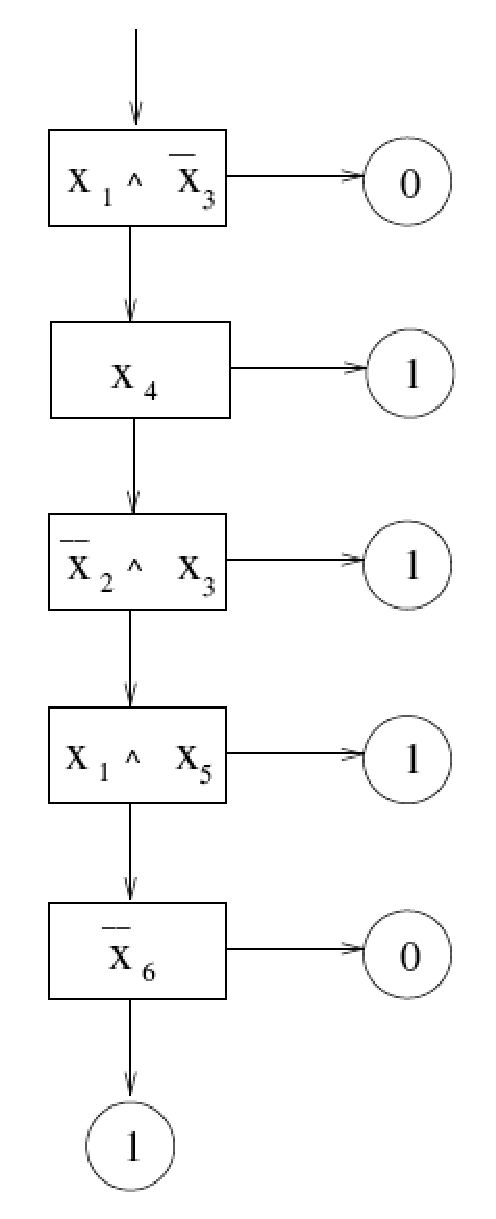
\includegraphics[width=1.35in]{fig-1.pdf}
\caption{A $2$-decision list.}
\label{fig:decision_list}
\end{center}
\end{figure}

A {\em $k$-decision list} over the variables $x_{1}, \ldots, x_{n}$ is
an ordered sequence $L=(c_{1}, b_{1}), \ldots, (c_{l},b_{l})$ and a
bit $b$, in which each $c_{i}$ is a conjunction of at most $k$
literals over $x_{1},\ldots, x_{n}$. The bit $b$ is called the {\em
  default} value, and $b_{i}$ is referred to as the bit {\em
  associated} with condition $c_{i}$. For any input $x \in \{0,
1\}^{n}$, $L(x)$ is defined to be the bit $b_{j}$, where $j$ is the
smallest index satisfying $c_{j}(x)=1$; if no such index exists, then
$L(x)=b$.

We denote by $k\mbox{\em -DL}$ the class of concepts that can be
represented by a $k$-decision list.


\begin{enumerate}
\item \relax[8 points] Show that if a concept $c$ can be represented
  as a $k$-decision list so can its complement, $\neg c$. You can show
  this by providing a $k$-decision list that represents $\neg c$,
  given $c = \{(c_{1},b_{1}), \ldots, (c_{l},b_{l}),b)$.

	\textbf{Response:} By leveraging \textit{a priori} from Ron Rivest in \textit{Learning Decision Lists}, we come to find that the solution is trivial and involves a minute manipulation of the decision list (DL). The complement $\neg c$ can be derived by negating all the leaves of the DL due to $k$-DL trees being closed under complementation. So, $$\neg c = \{(c_{1},\neg b_{1}), \ldots, (c_{l},\neg b_{l}),\neg b)$$

\item \relax[9 points] Use  Occam's Razor to show: \\
  For any constant $k \geq 1$, the class of $k$-decision lists is
  PAC-learnable. \newline\newline
  \textbf{Response:} We know that $k$-DL is polynomial-sized, that is, $|k \text{-DL(n)}|=O(3^{|C^n _k|}(|C^n _k|)!)$, where $C^n _k$ is the set of all conjuctions of size at most $k$ with literals drawn from $L_n$. Furthermore, each term can either be paired with 1 or 0 or missing in arbitrary order. Taking the 2-base lg:
  
  $$lg|k \text{-DL(n)}|=lg(O(3^{|C^n _k|}(|C^n _k|)!))$$
  Thus, for some constant $t$,
  $$lg|k \text{-DL(n)}|=O(n^t)$$
  Finally, we have shown that $k$-DL is PAC learnable in polynomial time for $k \geq 1$

\item \relax[8 points] Show that $1$-decision lists are a linearly
  separable functions. (Hint: Find a weight vector that will make the
  same predictions a given $1$-decision list.) \newline
  
  \textbf{Response:} For instance, suppose we have a conjunctive clause $c = x_1 ^ \neg x_2$. Now, let's consider a weight vector $w$ such that $w^T x$ yields the decision $d$. We can set $w$ to be the same as the conjunction $c$ itself, treating the literals as weights. Specifically, if the literal appears positively in $c$, we assign $w_i=1$; if it appears negatively, we assign $w_i=-1$. So w = [1, -1] for $c$. $$d = w^T x=x_1 - \neg x_2$$
	
\end{enumerate}





\end{document}

%%% Local Variables:
%%% mode: latex
%%% TeX-master: t
%%% End:
